\section{Triazole-linked autoinducer-antibiotic conjugates}

\subsection{Synthesis of autoinducer-antibiotic conjugate \compound{cmpd:HL2T4Cip}}

Test reactions using N$_3$-C$_2$-HSL \compound{cmpd:HL2N3} and the alkynyl ciprofloxacin derivative \compound{cmpd:Y4Cip} were performed to find conditions for the click reactions between the azido autoinducers and the alkynyl antibiotics (see \ref{tbl:HL2N3Y4Cip_opt} and \ref{sch:HL2N3Y4Cip_synth}). 
Stirring at r.t. had no effect even with an extended reaction time. Heating to 50 $^{\circ}$C did lead to slow formation of the product, but a mixture of the 1,4 \compound{cmpd:HL2T4Cip} and 1,5 \compound{cmpd:15HL2T4Cip} isomers was observed in an approximately 4:1 ratio by LCMS (see \ref{fig:14vs15}). Use of the ligand tris(3-hydroxypropyltriazolylmethyl)amine (THPTA) \compound{cmpd:THPTA} (see \ref{fig:THPTA}) led to some conversion at room temperature, however the reaction stopped before completion, probably due to oxidation of the Cu(I) catalytic species. When degassed solvent and an argon atmosphere were used the reaction proceeded to completion at room temperature in around 3 h.

\renewcommand{\arraystretch}{1.2}
\begin{table}[ht]
  \centering
\begin{tabular}{|p{0.3\textwidth}|p{0.3\textwidth}|}
\hline 
\textbf{Conditions} & \textbf{Outcome}\\ 
\hline 
\ce{CuSO4}$\cdot$\ce{H2O}, sodium ascorbate, \ce{H2O}, \textit{t}-BuOH, air, r.t., 7 d. & No reaction \\ 
\hline 
\ce{CuSO4}$\cdot$\ce{H2O}, sodium ascorbate, \ce{H2O}, \textit{t}-BuOH, air, 50 $^{\circ}$C, 5 d. & 1,3-Triazole product \compound{cmpd:HL2T4Cip} and 1,5 triazole impurity \compound{cmpd:15HL2T4Cip} 4:1 \\ 
\hline 
\ce{CuSO4}$\cdot$\ce{H2O}, sodium ascorbate, THPTA \compound{cmpd:THPTA}, \ce{H2O}, \textit{t}-BuOH, air, r.t., 3 h. & 1,3-Triazole product \compound{cmpd:HL2T4Cip} and starting materials \compound{cmpd:HL2N3} and  \compound{cmpd:Y4Cip}\\ 
\hline 
\ce{CuSO4}$\cdot$\ce{H2O}, sodium ascorbate, THPTA \compound{cmpd:THPTA}, \ce{H2O}, \textit{t}-BuOH, Ar, r.t., 3 h. & 1,3-Triazole product \compound{cmpd:HL2T4Cip} \\ 
\hline 
\end{tabular}
\caption{Conditions attempted for the synthesis of \compound{cmpd:HL2T4Cip} (see \ref{sch:HL2N3Y4Cip_synth}).\label{tbl:HL2N3Y4Cip_opt}} 
\end{table}

\begin{scheme}[H]
	\begin{center}
		\schemeref[HL2N3]{cmpd:HL2N3}
		\schemeref[hexpipcip]{cmpd:Y4Cip}
		\schemeref[HL2N3hexpipcip]{cmpd:HL2T4Cip}
		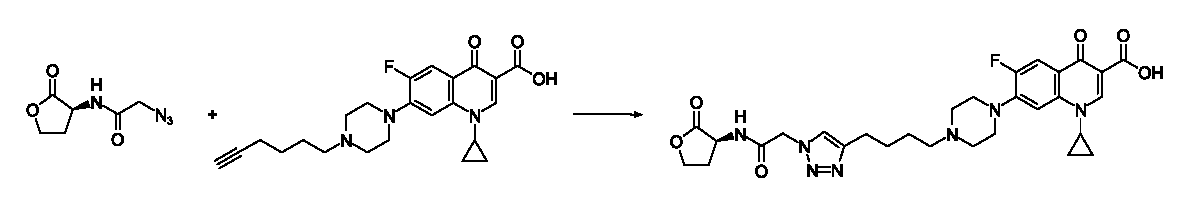
\includegraphics[scale=1]{HL2N3hexpipcip_synth}
		\caption{Synthesis of \compound{cmpd:HL2T4Cip}. For conditions see \ref{tbl:HL2N3Y4Cip_opt}. \label{sch:HL2N3Y4Cip_synth}}
	\end{center}
\end{scheme}


\begin{figure}[H]
	\begin{center}
		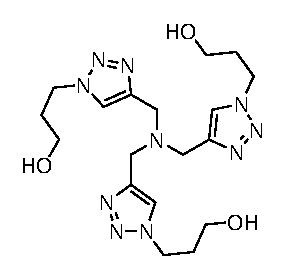
\includegraphics[scale=1]{THPTA}
		\caption{Tris[(1-benzyl-\textit{1H}-1,2,3-triazol-4-yl)methyl]amine (THPTA) \compound{cmpd:THPTA} .\label{fig:THPTA}}
	\end{center}
\end{figure}

\begin{figure}[H]
	\begin{center}
		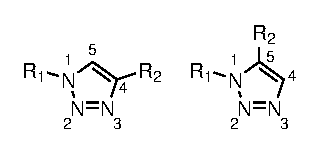
\includegraphics[scale=1]{14vs15}
		\caption{1,4 (left) and 1,5 (right) triazoles .\label{fig:14vs15}}
	\end{center}
\end{figure}

\subsection{Synthesis of the initial triazole-linked library}

Once conditions had been found for the click reaction, the synthesis of other conjugates was attempted. 
Two additional azides were kindly donated by members of the Spring group: 
the azido derivative of 3-oxo-C$_{12}$-HSL \compound{cmpd:HLO12N3} was synthesised by Ryan Howard, a master's student under my supervision\cite{Howard2015} and
the tail azide derivative of PQS \compound{cmpd:PQSN3} was synthesised by Ysobel Baker\cite{Baker2015} (see \ref{fig:furtherazs}).

\begin{figure}[H]
	\begin{center}
		\schemeref[HLO12N3]{cmpd:HLO12N3}
		\schemeref[PQSaz]{cmpd:PQSN3}
		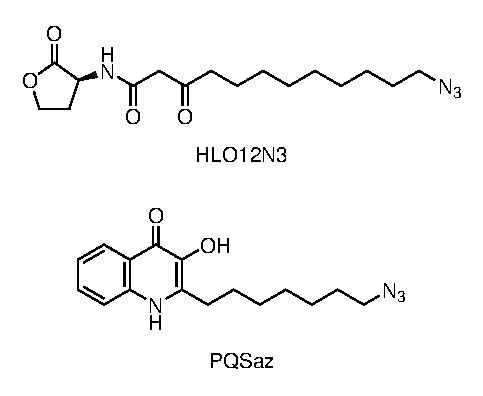
\includegraphics[scale=1]{furtherazs}
		\caption{Further azido autoinducer derivatives synthesised by Howard\cite{Howard2015} \compound{cmpd:HLO12N3} and Baker\cite{Baker2015} \compound{cmpd:PQSN3}.\label{fig:furtherazs}} 
	\end{center}
\end{figure}

Synthesis of the conjugates proved more difficult than expected; HSL derivatives hydrolysed upon attempted HPLC purification, the 3-oxo-C$_{12}$-HSL conjugates degraded, and the reaction was highly air-sensitive which led to stalling. The most reliable procedure was determined over the course of several reactions, and is shown in \ref{sec:click_general}.

Nonetheless, several conjugates were produced for testing. The results of the reactions are shown in \ref{tbl:Clicks_AHLs_Cip}, \ref{tbl:Clicks_Quins_Cip}, \ref{tbl:Clicks_AHLs_Tri} and \ref{tbl:Clicks_Quins_Tri}. It was intended that the failed reactions would be repeated, but as preliminary biological testing \todo{ref} proved unpromising it was decided that attention should be focused elsewhere.

\begin{scheme}[H]
	\begin{center}
		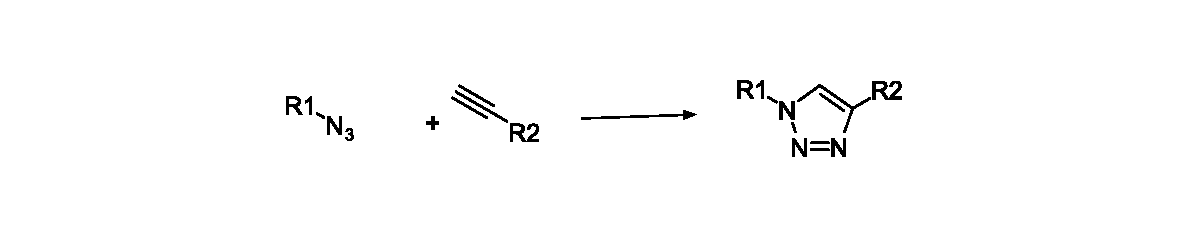
\includegraphics[scale=1]{QSAB_synth}
		\caption{General scheme for the click reaction, where R$_1$-N$_3$ is an azido autoinducer derivative and R$_2$-$\equiv$ is an alkynyl antibiotic derivative a)\ce{CuSO4}, sodium ascorbate, THPTA, \ce{H2O}, \textit{t}-BuOH.\label{sch:QSAB_synth}} 
	\end{center}
\end{scheme}

\begin{table}[H]
  \centering
  %\renewcommand{\arraystretch}{1.2}
\begin{tabular}{|m{0.10\textwidth}|M{0.60\textwidth}|m{0.14\textwidth}|m{0.06\textwidth}|}
\hline 
 \textbf{Starting materials} & \textbf{Product} & \textbf{Outcome} & \textbf{Yield} \\ 
\hline 
\compound{cmpd:HL2N3} and \compound{cmpd:Y4Cip} & \vspace{10px}\centering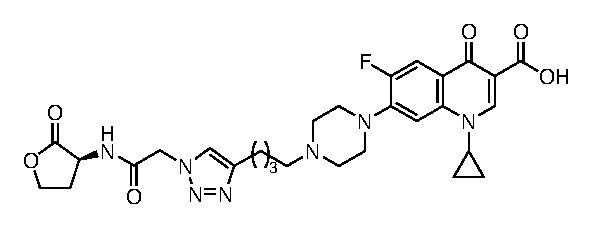
\includegraphics[scale=1]{HL2T4Cip_short} \\ \compound{cmpd:HL2T4Cip} & {\color{green}\cmark} Reaction complete by LCMS in 3 h. Purified by column chromatography (\ce{SiO2}, 0 - 20 \% MeOH/\ce{CH2Cl2}). & 29.6 \% \\ %LMO-1-084, LMO-1-092 (stalled. probably columned?)
\hline 
\compound{cmpd:HL4N3} and \compound{cmpd:Y4Cip} & \vspace{10px}\centering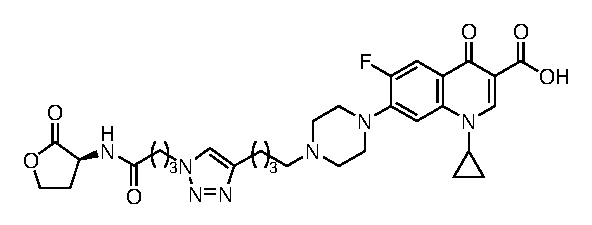
\includegraphics[scale=1]{HL4T4Cip_short} \\ \compound{cmpd:HL4T4Cip} & {\color{green}\cmark} Reaction complete by LCMS in 3 h. Purified by column chromatography (\ce{SiO2}, 0 - 20 \% MeOH/\ce{CH2Cl2}). & 46.8 \% \\  %LMO-1-094, (nothing written down, not sure about %MeOH.)
\hline 
\compound{cmpd:HL6N3} and \compound{cmpd:Y4Cip} & \vspace{10px}\centering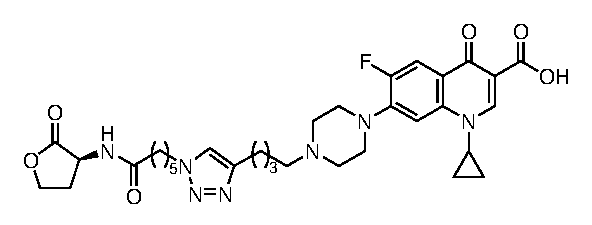
\includegraphics[scale=1]{HL6T4Cip_short} \\ \compound{cmpd:HL6T4Cip} & {\color{green}\cmark} Reaction complete by LCMS in 3 h. Purified by column chromatography (\ce{SiO2}, 0 - 20 \% MeOH/\ce{CH2Cl2}). & 38.0 \% \\ %LMO-1-090, LMO-1-093
\hline 
\compound{cmpd:HLO12N3} and \compound{cmpd:Y4Cip} & \vspace{10px}\centering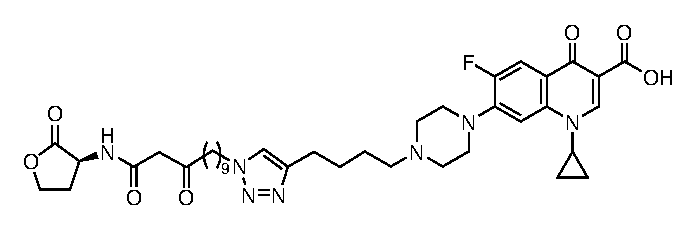
\includegraphics[scale=1]{HLO12T4Cip_short} \\ \compound{cmpd:HLO12T4Cip} & {\color{red}\xmark} Reaction complete by LCMS in 3.5 h, but product degraded when subjected to column chromatography (\ce{SiO2}, 20 \% MeOH/\ce{CH2Cl2}). & \\ %LMO-2-001
\hline
\end{tabular}
\caption{Click reactions attempted.\label{tbl:Clicks_AHLs_Cip}} 
\end{table}


\begin{table}[H]
  \centering
  %\renewcommand{\arraystretch}{1.2}
\begin{tabular}{|m{0.10\textwidth}|M{0.60\textwidth}|m{0.14\textwidth}|m{0.06\textwidth}|}
\hline 
 \textbf{Starting materials} & \textbf{Product} & \textbf{Outcome} & \textbf{Yield} \\ 
\hline 
\compound{cmpd:azHHQ} and \compound{cmpd:Y4Cip} & \vspace{10px}\centering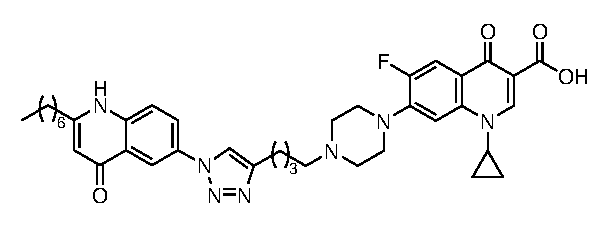
\includegraphics[scale=1]{6HHQT4Cip_short} \\ \compound{cmpd:6HHQT4Cip} & {\color{green}\cmark} Reaction complete by LCMS in 1.5 h. Purified by prep. HPLC. & 27.0 \% \\ %LMO-2-006
\hline
%\vspace{10px}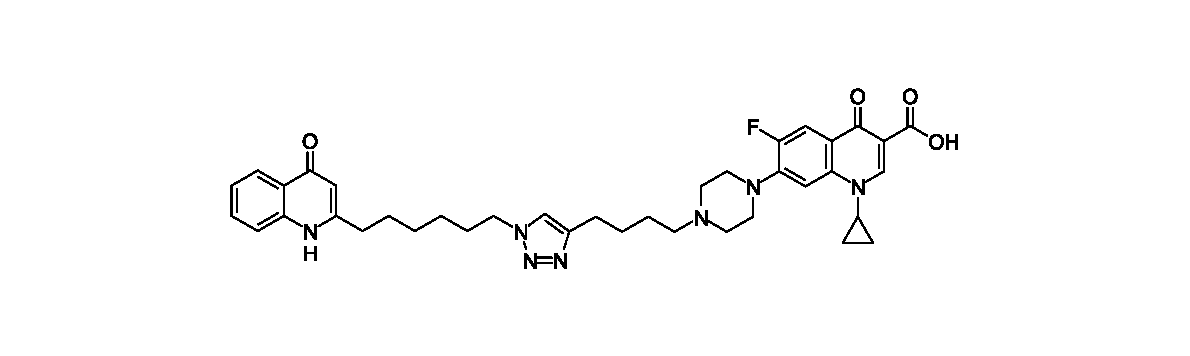
\includegraphics[scale=1]{HHQT4Cip} & {\color{red}\xmark} Reaction not attempted due to lack of starting material. \\
%\hline
\compound{cmpd:azPQS} and \compound{cmpd:Y4Cip} & \vspace{10px}\centering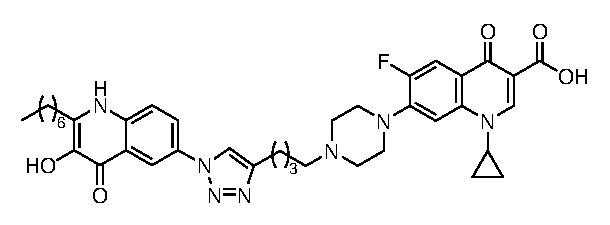
\includegraphics[scale=1]{6PQST4Cip_short} \\ \compound{cmpd:6PQST4Cip} & {\color{red}\xmark} Reaction did not go to completion by LCMS. Attempted purification by prep. HPLC but unsuccessful. &   \\ %LMO-2-009
\hline
\compound{cmpd:PQSN3} and \compound{cmpd:Y4Cip} & \vspace{10px}\centering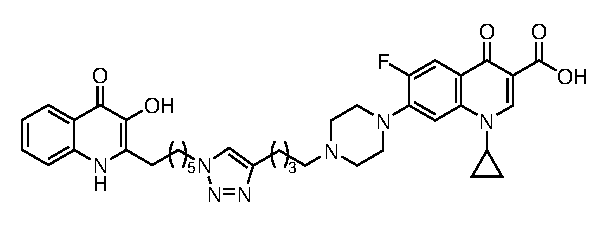
\includegraphics[scale=1]{PQST4Cip_short} \\ \compound{cmpd:PQST4Cip} & {\color{red}\xmark} No reaction seen by LCMS. &  \\ %LMO-2-007(didn't work?)
\hline 
\end{tabular}
\caption{Click reactions attempted.\label{tbl:Clicks_Quins_Cip}} 
\end{table}

\begin{table}[H]
  \centering
  %\renewcommand{\arraystretch}{1.2}
\begin{tabular}{|m{0.10\textwidth}|M{0.60\textwidth}|m{0.14\textwidth}|m{0.06\textwidth}|}
\hline 
 \textbf{Starting materials} & \textbf{Product} & \textbf{Outcome} & \textbf{Yield} \\ 
\hline 
\compound{cmpd:HL2N3} and \compound{cmpd:Y4Tri} & \vspace{10px}\centering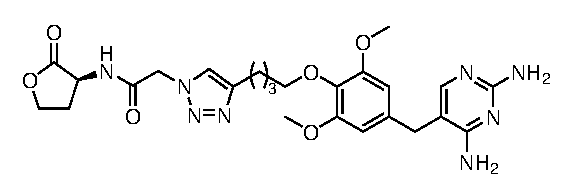
\includegraphics[scale=1]{HL2T4Tri_short} \\ \compound{cmpd:HL2T4Tri} & {\color{red}\xmark} Reaction complete by LCMS in 2 h, but lactone hydrolysed on prep. HPLC column. & \\ %LMO-1-084 (not sure what happened), LMO-2-004.
\hline 
\compound{cmpd:HL4N3} and \compound{cmpd:Y4Tri} & \vspace{10px}\centering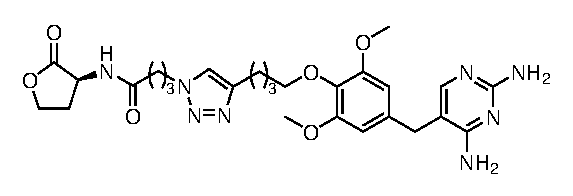
\includegraphics[scale=1]{HL4T4Tri_short} \\ \compound{cmpd:HL4T4Tri} & {\color{green}\cmark} Reaction complete by LCMS in 2 weeks (stalled). Purified by column chromatography (\ce{SiO2}, 20 \% MeOH/\ce{CH2Cl2}). & 16.8 \% \\ %LMO-1-090 (left 2 weeks)
\hline 
\compound{cmpd:HL6N3} and \compound{cmpd:Y4Tri} & \vspace{10px}\centering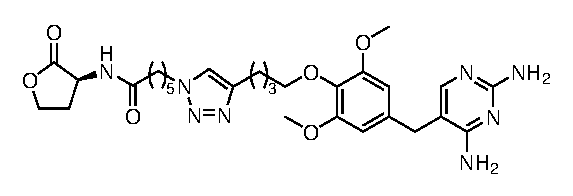
\includegraphics[scale=1]{HL6T4Tri_short} \\ \compound{cmpd:HL6T4Tri} & {\color{green}\cmark} Reaction complete by LCMS in 2 weeks (stalled). Purified by column chromatography (\ce{SiO2}, 20 \% MeOH/\ce{CH2Cl2}). & 26.8 \% \\ %LMO-1-090 (presumably columned)
\hline 
\compound{cmpd:HLO12N3} and \compound{cmpd:Y4Tri} & \vspace{10px}\centering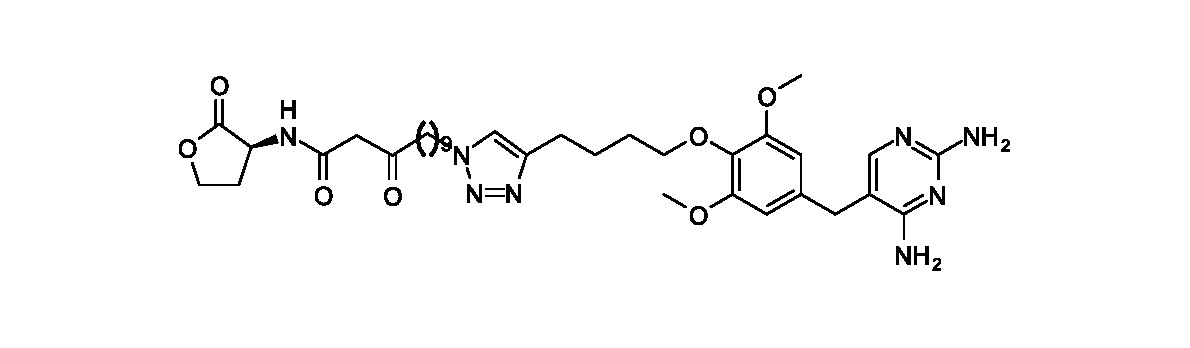
\includegraphics[scale=1]{HLO12T4Tri_short} \\ \compound{cmpd:HLO12T4Tri} & {\color{red}\xmark} Degraded during reaction. & \\  %LMO-1-090(left 3 weeks), LMO-1-091 (no outcome noted, probably degradation),
\hline
\end{tabular}
\caption{Click reactions attempted.\label{tbl:Clicks_AHLs_Tri}} 
\end{table}


\begin{table}[H]
  \centering
  %\renewcommand{\arraystretch}{1.2}
\begin{tabular}{|m{0.10\textwidth}|M{0.60\textwidth}|m{0.14\textwidth}|m{0.06\textwidth}|}
\hline 
 \textbf{Starting materials} & \textbf{Product} & \textbf{Outcome} & \textbf{Yield} \\ 
\hline 
\compound{cmpd:azHHQ} and \compound{cmpd:Y4Tri} & \vspace{10px}\centering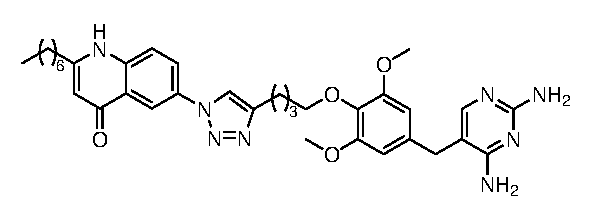
\includegraphics[scale=1]{6HHQT4Tri_short} \\ \compound{cmpd:6HHQT4Tri} & {\color{green}\cmark} Reaction complete by LCMS in 1.5 h. Purified by prep. HPLC. & 41.0 \% \\ %LMO-2-003, LMO-2-005
\hline
%\vspace{10px}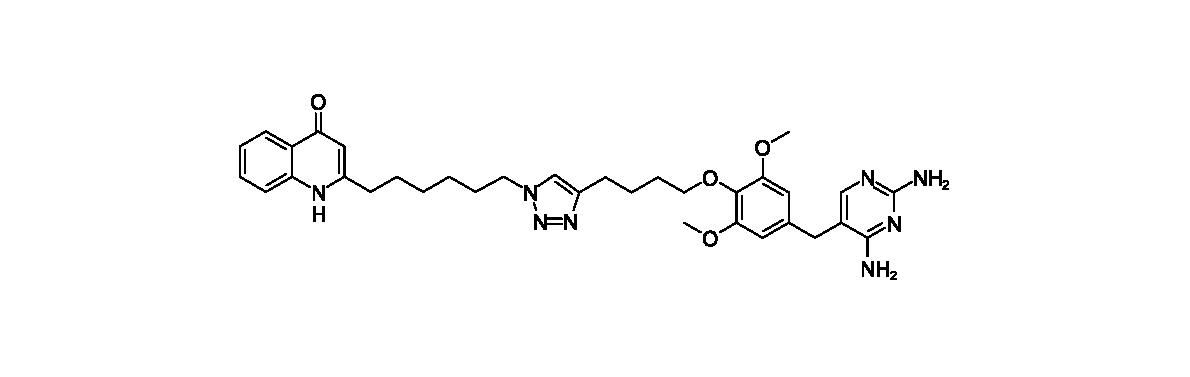
\includegraphics[scale=1]{HHQT4Tri} & {\color{red}\xmark} Reaction not attempted due to lack of starting material. \\ 
%\hline
\compound{cmpd:azPQS} and \compound{cmpd:Y4Tri} & \vspace{10px}\centering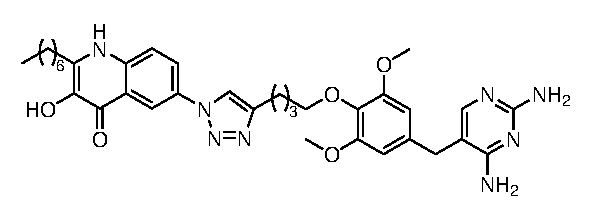
\includegraphics[scale=1]{6PQST4Tri_short} \\ \compound{cmpd:6PQST4Tri} & {\color{red}\xmark} Reaction did not go to completion by LCMS. Attempted purification by prep. HPLC but unsuccessful. &  \\ %LMO-2-008 
\hline
\compound{cmpd:PQSN3} and \compound{cmpd:Y4Tri} & \vspace{10px}\centering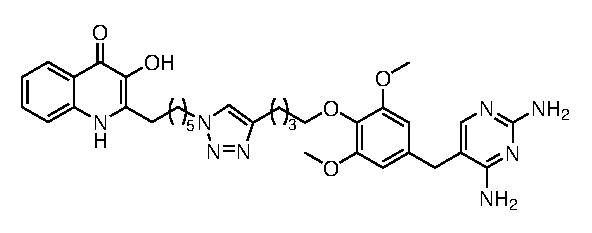
\includegraphics[scale=1]{PQST4Tri_short} \\ \compound{cmpd:PQST4Tri} & {\color{green}\cmark} Reaction complete by LCMS in 3 h. Purified by column chromatography (\ce{SiO2}, 20 \% MeOH/\ce{CH2Cl2}). & 18.3 \% \\ %LMO-1-090 (done but sample lost), LMO-2-002 
\hline 
\end{tabular}
\caption{Click reactions attempted.\label{tbl:Clicks_Quins_Tri}} 
\end{table}

